\appendix
\appendixpage*
\addappheadtotoc
\chapter{Basis matrix $W$ for the six survival-associated metagenes}
\label{app:sigs-w-matrix}
% latex table generated in R 3.1.1 by xtable 1.7-4 package
% Fri Dec  5 15:39:01 2014
\begin{longtable}{rrrrrrr}
  \hline
 & 1 & 2 & 3 & 4 & 5 & 6 \\ 
  \hline
PPY & 0.00 & 0.50 & 0.00 & 0.08 & 1.08 & 0.00 \\ 
  KRT6A & 0.14 & 0.00 & 0.12 & 0.00 & 0.00 & 0.47 \\ 
  KRT17 & 0.29 & 0.00 & 0.39 & 0.16 & 0.12 & 0.51 \\ 
  DHRS9 & 0.00 & 0.00 & 1.00 & 0.34 & 0.00 & 0.17 \\ 
  SPP1 & 0.03 & 0.08 & 0.00 & 1.04 & 0.31 & 0.74 \\ 
  ADH1A & 0.07 & 0.44 & 0.01 & 0.10 & 0.66 & 0.00 \\ 
  IGLL3P & 0.17 & 0.15 & 0.00 & 0.00 & 0.76 & 0.00 \\ 
  DKK1 & 0.48 & 0.00 & 0.30 & 0.18 & 0.00 & 0.02 \\ 
  APCS & 0.00 & 0.03 & 0.16 & 0.10 & 0.16 & 0.35 \\ 
  CST6 & 0.07 & 0.00 & 0.20 & 0.00 & 0.07 & 0.63 \\ 
  ANGPTL4 & 0.18 & 0.00 & 0.42 & 0.05 & 0.03 & 0.39 \\ 
  KRT7 & 0.46 & 0.00 & 0.56 & 0.00 & 0.14 & 0.44 \\ 
  PLAU & 0.21 & 0.00 & 0.28 & 0.00 & 0.02 & 0.88 \\ 
  SCGB2A1 & 0.00 & 0.83 & 0.00 & 0.18 & 0.15 & 0.00 \\ 
  CCL19 & 0.00 & 0.00 & 0.00 & 0.00 & 0.95 & 0.00 \\ 
  CYP2S1 & 0.32 & 1.02 & 0.15 & 0.00 & 0.09 & 0.00 \\ 
  SLC2A1 & 0.18 & 0.12 & 1.00 & 0.41 & 0.00 & 0.70 \\ 
  ADM & 0.00 & 0.00 & 0.52 & 0.51 & 0.00 & 0.36 \\ 
  FAM83A & 0.25 & 0.00 & 0.12 & 0.00 & 0.00 & 0.22 \\ 
  FGG & 0.05 & 0.04 & 0.00 & 0.14 & 0.01 & 0.22 \\ 
  KRT6C & 0.12 & 0.00 & 0.00 & 0.00 & 0.00 & 0.16 \\ 
  PHACTR3 & 0.15 & 0.00 & 0.32 & 0.14 & 0.00 & 0.07 \\ 
  C9orf152 & 0.21 & 1.37 & 0.00 & 0.35 & 0.02 & 0.00 \\ 
  ALOX5AP & 0.05 & 0.01 & 0.01 & 1.27 & 0.34 & 0.71 \\ 
  DCBLD2 & 0.40 & 0.00 & 0.12 & 0.00 & 0.14 & 0.84 \\ 
  CIDEC & 0.03 & 0.00 & 0.43 & 0.28 & 0.00 & 0.00 \\ 
  FGB & 0.00 & 0.00 & 0.02 & 0.32 & 0.00 & 0.08 \\ 
  SERPINB3 & 0.00 & 0.00 & 0.18 & 0.18 & 0.00 & 0.05 \\ 
  SLC16A3 & 0.13 & 0.38 & 1.10 & 0.42 & 0.00 & 1.00 \\ 
  FST & 0.00 & 0.00 & 0.16 & 0.00 & 0.04 & 0.49 \\ 
  CAV1 & 0.42 & 0.00 & 0.19 & 0.08 & 0.27 & 0.84 \\ 
  TGFBI & 0.19 & 0.00 & 0.15 & 0.19 & 0.05 & 1.00 \\ 
  COL12A1 & 0.00 & 0.13 & 0.03 & 0.53 & 0.19 & 1.65 \\ 
  SLC2A3 & 0.00 & 0.00 & 0.34 & 0.76 & 0.33 & 0.72 \\ 
  SUGCT & 0.00 & 0.03 & 0.00 & 0.63 & 0.13 & 0.93 \\ 
  IL1R2 & 0.04 & 0.25 & 0.43 & 0.23 & 0.00 & 0.06 \\ 
  TCEA3 & 0.00 & 0.89 & 0.26 & 0.09 & 0.62 & 0.00 \\ 
  RAP1GAP & 0.00 & 1.01 & 0.47 & 0.28 & 0.75 & 0.00 \\ 
  PXDN & 0.00 & 0.00 & 0.38 & 0.59 & 0.31 & 1.19 \\ 
  FRZB & 0.09 & 0.24 & 0.00 & 0.54 & 1.50 & 0.00 \\ 
  IL20RB & 0.26 & 0.00 & 0.31 & 0.00 & 0.00 & 0.68 \\ 
  PLEKHS1 & 0.00 & 0.64 & 0.34 & 0.09 & 0.28 & 0.02 \\ 
  HSPB6 & 0.00 & 0.15 & 0.13 & 0.00 & 1.31 & 0.31 \\ 
  KANK4 & 0.00 & 0.00 & 0.20 & 0.47 & 0.00 & 1.23 \\ 
  COL7A1 & 0.00 & 0.00 & 0.59 & 0.00 & 0.00 & 0.59 \\ 
  C5orf46 & 0.00 & 0.00 & 0.00 & 1.06 & 0.13 & 1.04 \\ 
  VSTM2L & 0.32 & 0.00 & 0.94 & 0.00 & 0.05 & 0.07 \\ 
  PTGES & 0.57 & 0.02 & 0.57 & 0.07 & 0.00 & 0.56 \\ 
  FSCN1 & 0.37 & 0.07 & 1.06 & 0.13 & 0.14 & 0.74 \\ 
  CTSV & 0.30 & 0.04 & 0.26 & 0.02 & 0.02 & 0.18 \\ 
  SPOCK1 & 0.12 & 0.00 & 0.03 & 0.52 & 0.34 & 1.27 \\ 
  RGS5 & 0.00 & 0.43 & 0.05 & 0.08 & 0.58 & 0.09 \\ 
  PHLDA1 & 0.08 & 0.14 & 0.72 & 0.13 & 0.62 & 1.50 \\ 
  IGFBP1 & 0.27 & 0.00 & 0.23 & 0.03 & 0.00 & 0.01 \\ 
  BAMBI & 0.11 & 0.00 & 0.84 & 0.39 & 0.24 & 0.17 \\ 
  FLRT3 & 0.79 & 0.13 & 0.51 & 0.28 & 0.22 & 0.31 \\ 
  DSG3 & 0.18 & 0.00 & 0.21 & 0.00 & 0.00 & 0.54 \\ 
  ANGPTL2 & 0.00 & 0.00 & 0.37 & 0.87 & 0.18 & 0.92 \\ 
  ST6GAL1 & 0.17 & 0.84 & 0.00 & 0.23 & 0.67 & 0.09 \\ 
  SLC40A1 & 0.00 & 0.89 & 0.00 & 0.58 & 0.24 & 0.16 \\ 
  EMP3 & 0.25 & 0.00 & 0.46 & 0.16 & 0.22 & 0.56 \\ 
  RAB31 & 0.11 & 0.00 & 0.26 & 0.87 & 0.76 & 1.19 \\ 
  ST6GALNAC1 & 0.04 & 1.00 & 0.08 & 0.12 & 0.00 & 0.10 \\ 
  ACKR3 & 0.00 & 0.00 & 0.38 & 0.36 & 0.21 & 0.58 \\ 
  SLC12A2 & 0.04 & 0.91 & 0.34 & 0.10 & 0.49 & 0.18 \\ 
  ANKRD22 & 0.41 & 1.35 & 0.17 & 0.27 & 0.04 & 0.22 \\ 
  ENO2 & 0.36 & 0.34 & 0.79 & 0.03 & 0.00 & 0.94 \\ 
  EPHX2 & 0.00 & 0.59 & 0.11 & 0.17 & 0.68 & 0.00 \\ 
  MCEMP1 & 0.00 & 0.00 & 0.00 & 0.61 & 0.00 & 0.30 \\ 
  CDA & 0.29 & 0.00 & 0.34 & 0.00 & 0.00 & 0.70 \\ 
  PLIN2 & 0.31 & 0.00 & 0.08 & 1.02 & 0.47 & 0.21 \\ 
  SERPINH1 & 0.00 & 0.01 & 0.39 & 0.22 & 0.43 & 1.02 \\ 
  FAM134B & 0.00 & 0.82 & 0.00 & 0.23 & 0.21 & 0.00 \\ 
  NFIX & 0.00 & 0.88 & 0.14 & 0.00 & 1.39 & 0.80 \\ 
  LYNX1 & 0.03 & 0.00 & 0.26 & 0.17 & 0.00 & 0.10 \\ 
  LDHA & 0.65 & 0.47 & 0.00 & 0.32 & 0.05 & 1.17 \\ 
  SOD2 & 0.58 & 0.12 & 0.00 & 0.47 & 0.40 & 0.17 \\ 
  PCDH20 & 0.00 & 0.43 & 0.00 & 0.15 & 0.00 & 0.00 \\ 
  ITGA5 & 0.00 & 0.00 & 0.48 & 0.27 & 0.12 & 0.68 \\ 
  ZNF185 & 0.25 & 0.17 & 1.02 & 0.48 & 0.00 & 0.72 \\ 
  PLOD2 & 0.15 & 0.09 & 0.24 & 0.29 & 0.17 & 0.89 \\ 
  TNFRSF6B & 0.63 & 0.00 & 0.07 & 0.18 & 0.00 & 0.39 \\ 
  MME & 0.00 & 0.00 & 0.06 & 0.45 & 0.04 & 0.58 \\ 
  MRAP2 & 0.04 & 0.78 & 0.00 & 0.22 & 0.23 & 0.00 \\ 
  PLAC9 & 0.07 & 0.00 & 0.00 & 0.11 & 1.29 & 0.08 \\ 
  ERRFI1 & 0.16 & 0.03 & 0.55 & 0.35 & 0.29 & 0.79 \\ 
  PP7080 & 0.10 & 0.97 & 0.00 & 0.04 & 0.00 & 0.00 \\ 
  DSG2 & 0.43 & 0.57 & 0.18 & 0.51 & 0.04 & 0.71 \\ 
  APCDD1 & 0.00 & 0.14 & 0.15 & 0.13 & 0.60 & 0.84 \\ 
  PRKCDBP & 0.26 & 0.00 & 1.02 & 0.51 & 0.26 & 0.59 \\ 
  SULF2 & 0.17 & 0.15 & 0.46 & 0.19 & 0.39 & 0.77 \\ 
  TUBA1C & 1.31 & 0.55 & 0.54 & 0.53 & 0.27 & 0.50 \\ 
  PCOLCE2 & 0.00 & 0.01 & 0.12 & 0.54 & 0.00 & 0.05 \\ 
  LAMA5 & 0.37 & 0.08 & 1.02 & 0.00 & 0.34 & 0.18 \\ 
  P4HA1 & 0.04 & 0.10 & 0.41 & 0.84 & 0.00 & 0.55 \\ 
  RASL11B & 0.00 & 0.19 & 0.07 & 0.22 & 1.21 & 0.31 \\ 
  KYNU & 0.61 & 0.09 & 0.07 & 0.54 & 0.00 & 0.28 \\ 
  CTSL & 0.39 & 0.00 & 0.20 & 1.18 & 0.47 & 0.22 \\ 
  MARCKSL1 & 0.15 & 1.34 & 0.30 & 0.00 & 0.00 & 0.26 \\ 
  PRC1 & 0.96 & 0.35 & 0.04 & 0.04 & 0.00 & 0.32 \\ 
  C1QTNF6 & 0.00 & 0.00 & 0.59 & 0.62 & 0.22 & 0.97 \\ 
  CCR7 & 0.06 & 0.00 & 0.00 & 0.00 & 1.05 & 0.00 \\ 
  HRASLS2 & 0.33 & 0.00 & 0.30 & 0.22 & 0.00 & 0.00 \\ 
  CHN2 & 0.00 & 0.50 & 0.00 & 0.34 & 0.44 & 0.00 \\ 
  PYGL & 0.08 & 0.00 & 0.31 & 0.34 & 0.14 & 0.74 \\ 
  MELK & 1.02 & 0.29 & 0.00 & 0.23 & 0.01 & 0.22 \\ 
  LOX & 0.21 & 0.00 & 0.08 & 0.39 & 0.09 & 0.92 \\ 
  CDC45 & 0.96 & 0.08 & 0.11 & 0.34 & 0.03 & 0.00 \\ 
  AXIN2 & 0.00 & 0.52 & 0.44 & 0.13 & 0.81 & 0.29 \\ 
  ATL3 & 0.64 & 0.03 & 0.16 & 0.49 & 0.25 & 0.29 \\ 
  CAMK1G & 0.09 & 0.24 & 0.00 & 0.03 & 0.88 & 0.00 \\ 
  ABLIM1 & 0.01 & 0.91 & 0.32 & 0.00 & 0.61 & 0.34 \\ 
  TRIM2 & 0.13 & 1.15 & 0.31 & 0.31 & 0.36 & 0.00 \\ 
  TWIST1 & 0.00 & 0.00 & 0.20 & 0.91 & 0.12 & 1.20 \\ 
  ARSD & 0.15 & 1.24 & 0.19 & 0.00 & 0.22 & 0.14 \\ 
  CEBPB & 0.07 & 0.07 & 1.29 & 0.53 & 0.51 & 0.81 \\ 
  CEP55 & 1.42 & 0.33 & 0.00 & 0.17 & 0.00 & 0.46 \\ 
  GINS2 & 1.08 & 0.18 & 0.39 & 0.07 & 0.00 & 0.00 \\ 
  MCM4 & 1.28 & 0.14 & 0.31 & 0.03 & 0.01 & 0.13 \\ 
  PPP1R3C & 0.00 & 0.02 & 0.13 & 0.37 & 0.03 & 0.26 \\ 
  MTRNR2L1 & 0.28 & 0.56 & 0.49 & 0.07 & 0.55 & 0.00 \\ 
  CDK12 & 0.19 & 0.28 & 0.00 & 0.08 & 0.83 & 0.00 \\ 
  BIRC5 & 1.38 & 0.17 & 0.37 & 0.55 & 0.00 & 0.24 \\ 
  SPHK1 & 0.26 & 0.00 & 0.27 & 0.09 & 0.62 & 1.41 \\ 
  A4GALT & 0.03 & 0.00 & 1.30 & 0.08 & 0.36 & 0.52 \\ 
  ICAM2 & 0.50 & 0.20 & 0.48 & 0.31 & 0.40 & 0.13 \\ 
  ANKRD37 & 0.06 & 0.18 & 0.22 & 0.72 & 0.01 & 0.57 \\ 
  STK39 & 0.15 & 1.00 & 0.24 & 0.14 & 0.08 & 0.12 \\ 
  ASPM & 1.17 & 0.39 & 0.20 & 0.17 & 0.04 & 0.04 \\ 
  PFKFB4 & 0.55 & 0.22 & 0.68 & 0.43 & 0.14 & 0.29 \\ 
  IDH2 & 0.71 & 0.43 & 0.40 & 0.21 & 0.33 & 0.23 \\ 
  SGSM1 & 0.00 & 0.93 & 0.08 & 0.02 & 0.84 & 0.00 \\ 
  SELENBP1 & 0.00 & 1.20 & 0.36 & 0.20 & 0.26 & 0.00 \\ 
  P4HA2 & 0.32 & 0.17 & 0.12 & 0.54 & 0.11 & 0.74 \\ 
  LMO3 & 0.00 & 0.11 & 0.00 & 0.01 & 1.18 & 0.01 \\ 
  KLHL5 & 0.42 & 0.16 & 0.00 & 0.35 & 0.70 & 1.14 \\ 
  HIPK2 & 0.26 & 1.25 & 0.07 & 0.24 & 0.52 & 0.00 \\ 
  NAMPT & 0.34 & 0.00 & 0.05 & 0.75 & 0.32 & 0.35 \\ 
  NCAPG & 1.61 & 0.44 & 0.00 & 0.00 & 0.00 & 0.52 \\ 
  PLOD1 & 0.06 & 0.00 & 1.21 & 0.75 & 0.37 & 0.80 \\ 
  C2orf70 & 0.11 & 1.09 & 0.02 & 0.00 & 0.00 & 0.00 \\ 
  RERGL & 0.24 & 0.00 & 0.00 & 0.11 & 1.18 & 0.00 \\ 
  CFDP1 & 0.35 & 0.55 & 0.74 & 0.67 & 0.00 & 0.26 \\ 
  RACGAP1 & 1.37 & 0.37 & 0.14 & 0.19 & 0.07 & 0.33 \\ 
  SNRPB & 0.99 & 0.08 & 0.41 & 0.90 & 0.02 & 0.00 \\ 
  CLEC3B & 0.06 & 0.07 & 0.12 & 0.01 & 0.81 & 0.00 \\ 
  ANLN & 1.17 & 0.24 & 0.08 & 0.08 & 0.00 & 0.72 \\ 
  ZFPM1 & 0.00 & 1.22 & 0.29 & 0.00 & 0.43 & 0.15 \\ 
  UPP1 & 0.55 & 0.00 & 0.79 & 0.43 & 0.16 & 0.11 \\ 
  AURKB & 1.00 & 0.11 & 0.14 & 0.00 & 0.01 & 0.00 \\ 
  SYNE2 & 0.00 & 0.88 & 0.24 & 0.00 & 0.28 & 0.28 \\ 
  SOBP & 0.00 & 0.20 & 0.81 & 0.10 & 1.36 & 0.00 \\ 
  GAPDH & 0.48 & 0.39 & 0.83 & 0.24 & 0.00 & 0.72 \\ 
  SERTAD2 & 0.29 & 0.14 & 0.90 & 0.99 & 0.49 & 0.44 \\ 
  TPX2 & 1.32 & 0.15 & 0.04 & 0.15 & 0.04 & 0.11 \\ 
  POC1A & 1.38 & 0.33 & 0.32 & 0.47 & 0.00 & 0.00 \\ 
  PDLIM7 & 0.20 & 0.00 & 0.41 & 0.37 & 0.11 & 0.68 \\ 
  TSTD1 & 0.17 & 1.22 & 0.48 & 0.07 & 0.45 & 0.02 \\ 
  PLIN3 & 0.34 & 0.26 & 0.97 & 0.93 & 0.14 & 0.41 \\ 
  IL33 & 0.24 & 0.04 & 0.00 & 0.13 & 0.68 & 0.00 \\ 
  CA8 & 0.00 & 0.69 & 0.05 & 0.01 & 0.05 & 0.00 \\ 
  SAMD5 & 0.13 & 0.54 & 0.00 & 0.00 & 0.09 & 0.00 \\ 
  NFIA & 0.12 & 0.84 & 0.00 & 0.39 & 1.50 & 0.27 \\ 
  KCTD5 & 0.38 & 0.51 & 1.13 & 0.61 & 0.00 & 0.00 \\ 
  CCNB1 & 1.43 & 0.46 & 0.13 & 0.25 & 0.02 & 0.36 \\ 
  TM9SF3 & 0.00 & 1.08 & 0.22 & 0.00 & 0.16 & 0.21 \\ 
  KIF20A & 1.37 & 0.29 & 0.21 & 0.23 & 0.00 & 0.29 \\ 
  PROSER2 & 0.93 & 0.18 & 0.40 & 0.37 & 0.27 & 0.40 \\ 
  COLGALT1 & 0.40 & 0.16 & 0.62 & 0.43 & 0.16 & 0.88 \\ 
  PPM1H & 0.00 & 0.85 & 0.46 & 0.27 & 0.24 & 0.00 \\ 
  NCAPD2 & 1.38 & 0.41 & 0.16 & 0.12 & 0.20 & 0.32 \\ 
  PREP & 0.06 & 0.98 & 0.30 & 0.20 & 0.02 & 0.00 \\ 
  DPY19L1 & 0.34 & 0.36 & 0.30 & 0.54 & 0.08 & 0.51 \\ 
  CKAP2L & 1.78 & 0.22 & 0.27 & 0.03 & 0.00 & 0.09 \\ 
  ZBED2 & 0.16 & 0.00 & 0.18 & 0.00 & 0.00 & 0.64 \\ 
  MIR99AHG & 0.04 & 0.28 & 0.39 & 0.45 & 1.79 & 0.22 \\ 
  P2RY2 & 0.18 & 0.03 & 0.77 & 0.22 & 0.00 & 0.50 \\ 
  KIF2C & 0.80 & 0.13 & 0.11 & 0.01 & 0.00 & 0.00 \\ 
  PPP1R14B & 0.37 & 0.26 & 0.78 & 0.00 & 0.37 & 0.59 \\ 
  GPC3 & 0.10 & 0.23 & 0.00 & 0.00 & 1.27 & 0.00 \\ 
  MAP3K8 & 0.20 & 0.00 & 0.07 & 0.31 & 0.56 & 0.43 \\ 
  NMB & 0.21 & 0.19 & 0.66 & 0.79 & 0.00 & 0.36 \\ 
  RAVER2 & 0.20 & 0.91 & 0.05 & 0.09 & 0.27 & 0.06 \\ 
  SPIN4 & 0.85 & 0.32 & 0.80 & 0.39 & 0.22 & 0.40 \\ 
  AMOT & 0.07 & 0.82 & 0.14 & 0.52 & 0.43 & 0.57 \\ 
  POP5 & 0.56 & 0.51 & 1.52 & 0.23 & 0.11 & 0.18 \\ 
  COLGALT2 & 0.00 & 0.60 & 0.00 & 0.02 & 0.00 & 0.00 \\ 
  DCUN1D5 & 1.36 & 0.08 & 0.00 & 0.86 & 0.96 & 0.72 \\ 
  DNAJC9 & 0.78 & 0.11 & 0.37 & 0.12 & 0.13 & 0.15 \\ 
  KCTD10 & 0.38 & 0.13 & 0.29 & 0.44 & 0.51 & 0.79 \\ 
  MIF & 0.43 & 0.33 & 0.96 & 0.44 & 0.00 & 0.68 \\ 
  SLAMF9 & 0.04 & 0.00 & 0.00 & 0.67 & 0.00 & 0.07 \\ 
  MCOLN2 & 0.20 & 0.28 & 0.00 & 0.00 & 0.94 & 0.00 \\ 
  CSNK1D & 0.21 & 0.38 & 1.56 & 0.48 & 0.16 & 0.23 \\ 
  TMED1 & 0.26 & 0.34 & 1.15 & 0.83 & 0.49 & 0.28 \\ 
  CADPS2 & 0.26 & 1.29 & 0.00 & 0.55 & 1.02 & 0.57 \\ 
  MEOX1 & 0.00 & 0.05 & 0.16 & 0.04 & 0.96 & 0.00 \\ 
  GIMAP2 & 0.15 & 0.72 & 0.00 & 0.66 & 0.77 & 0.00 \\ 
  RFC5 & 1.08 & 0.24 & 0.00 & 0.52 & 0.16 & 0.31 \\ 
  CARHSP1 & 0.75 & 0.53 & 0.87 & 0.90 & 0.26 & 0.00 \\ 
  SLC15A1 & 0.00 & 0.00 & 0.48 & 0.00 & 0.06 & 0.06 \\ 
  BCL11B & 0.20 & 0.92 & 0.23 & 0.24 & 0.42 & 0.00 \\ 
  CDK2 & 1.06 & 0.25 & 0.01 & 0.52 & 0.33 & 0.33 \\ 
  KIAA1549L & 0.38 & 0.08 & 0.26 & 0.66 & 0.15 & 0.64 \\ 
  HJURP & 1.33 & 0.24 & 0.23 & 0.02 & 0.00 & 0.00 \\ 
  FYN & 0.01 & 0.52 & 0.12 & 0.13 & 1.69 & 0.87 \\ 
  RNF103 & 0.03 & 1.25 & 0.17 & 0.55 & 0.29 & 0.06 \\ 
  ACYP2 & 0.25 & 0.89 & 0.00 & 0.23 & 0.85 & 0.41 \\ 
  CD70 & 0.09 & 0.00 & 0.21 & 0.36 & 0.00 & 0.43 \\ 
  PPAPDC1A & 0.00 & 0.00 & 0.00 & 0.76 & 0.00 & 1.22 \\ 
  TPD52L2 & 0.63 & 0.16 & 1.31 & 0.65 & 0.44 & 0.23 \\ 
  TOM1 & 0.00 & 0.10 & 1.49 & 0.81 & 0.68 & 0.52 \\ 
  DERA & 1.18 & 0.20 & 0.46 & 0.60 & 0.29 & 0.32 \\ 
  TREM1 & 0.05 & 0.00 & 0.09 & 0.71 & 0.00 & 0.30 \\ 
  UFC1 & 0.00 & 1.19 & 0.25 & 0.47 & 0.30 & 0.00 \\ 
  TCTA & 0.00 & 0.75 & 0.82 & 0.09 & 0.98 & 0.02 \\ 
  ALDH5A1 & 0.10 & 0.99 & 0.55 & 0.06 & 0.90 & 0.22 \\ 
  KNTC1 & 1.07 & 0.14 & 0.44 & 0.08 & 0.15 & 0.28 \\ 
  XXYLT1 & 0.24 & 0.00 & 1.05 & 1.08 & 0.46 & 0.87 \\ 
  SMOX & 0.37 & 0.29 & 1.43 & 1.00 & 0.18 & 0.00 \\ 
  ARFGAP3 & 0.03 & 0.30 & 0.54 & 0.84 & 0.49 & 0.54 \\ 
  SEPW1 & 0.03 & 0.95 & 1.24 & 0.00 & 0.63 & 0.56 \\ 
  ANKLE2 & 0.75 & 0.14 & 0.62 & 0.51 & 0.19 & 0.38 \\ 
  TLE4 & 0.05 & 0.88 & 0.07 & 0.33 & 0.90 & 0.47 \\ 
  RBMS2 & 0.61 & 0.15 & 0.00 & 0.40 & 0.32 & 0.89 \\ 
  AKR1A1 & 0.25 & 1.08 & 0.26 & 0.29 & 0.66 & 0.45 \\ 
  RERE & 0.05 & 0.74 & 0.62 & 0.00 & 0.99 & 0.42 \\ 
  ATAD2 & 0.94 & 0.07 & 0.11 & 0.03 & 0.11 & 0.31 \\ 
  SPOCD1 & 0.00 & 0.00 & 0.18 & 0.21 & 0.00 & 0.76 \\ 
  DYNC2H1 & 0.00 & 1.61 & 0.15 & 0.00 & 0.76 & 0.67 \\ 
  CAPN6 & 0.00 & 0.75 & 0.00 & 0.23 & 0.64 & 0.00 \\ 
  RPIA & 0.46 & 1.35 & 0.22 & 0.19 & 0.46 & 0.00 \\ 
  P2RY8 & 0.23 & 0.07 & 0.00 & 0.28 & 1.66 & 0.00 \\ 
  ARHGEF19 & 0.08 & 0.08 & 1.20 & 0.52 & 0.45 & 0.51 \\ 
  ARL4C & 0.00 & 0.02 & 0.30 & 0.49 & 0.30 & 1.23 \\ 
  CHAF1B & 0.99 & 0.30 & 0.20 & 0.02 & 0.52 & 0.10 \\ 
  FHDC1 & 0.18 & 1.24 & 0.22 & 0.02 & 0.00 & 0.05 \\ 
  POLA2 & 0.84 & 0.22 & 0.33 & 0.13 & 0.21 & 0.00 \\ 
  AGRP & 0.00 & 0.00 & 0.00 & 0.68 & 0.00 & 0.17 \\ 
  RPA2 & 0.47 & 0.70 & 0.70 & 0.41 & 1.42 & 0.24 \\ 
  MRPL24 & 0.16 & 1.13 & 0.22 & 0.12 & 0.22 & 0.18 \\ 
  PRDM16 & 0.00 & 1.12 & 0.00 & 0.00 & 0.53 & 0.09 \\ 
  POU2AF1 & 0.06 & 0.47 & 0.00 & 0.00 & 0.92 & 0.00 \\ 
  MC1R & 0.10 & 0.13 & 1.08 & 0.87 & 0.47 & 0.13 \\ 
  TNFRSF17 & 0.03 & 0.05 & 0.00 & 0.08 & 0.58 & 0.00 \\ 
  FAH & 0.68 & 0.42 & 0.36 & 0.21 & 0.32 & 0.39 \\ 
  HSP90B1 & 0.53 & 0.46 & 0.78 & 0.90 & 0.30 & 0.38 \\ 
  TRAPPC2 & 0.51 & 1.08 & 0.00 & 0.49 & 0.62 & 0.14 \\ 
  ARHGAP24 & 0.06 & 1.06 & 0.02 & 0.75 & 1.10 & 0.62 \\ 
  ABHD16A & 0.66 & 0.72 & 0.00 & 0.00 & 0.52 & 0.22 \\ 
  TMTC4 & 0.00 & 1.29 & 0.33 & 0.21 & 0.20 & 0.28 \\ 
  SCYL2 & 0.70 & 0.39 & 0.00 & 0.98 & 0.41 & 0.96 \\ 
  TOR2A & 0.00 & 0.99 & 0.48 & 0.20 & 0.53 & 0.00 \\ 
  IKBIP & 0.29 & 0.00 & 0.30 & 1.12 & 0.15 & 0.47 \\ 
  DENND1A & 0.82 & 0.00 & 0.25 & 0.19 & 0.00 & 0.18 \\ 
  BCKDK & 0.22 & 0.29 & 0.87 & 1.07 & 0.40 & 0.11 \\ 
  KIAA0513 & 0.08 & 1.04 & 0.17 & 0.32 & 0.59 & 0.00 \\ 
  CNNM1 & 0.00 & 0.87 & 0.41 & 0.00 & 0.09 & 0.00 \\ 
  VPS35 & 0.39 & 1.39 & 0.00 & 0.53 & 0.00 & 0.25 \\ 
  ZPLD1 & 0.00 & 0.00 & 0.19 & 0.03 & 0.03 & 0.11 \\ 
  CHEK1 & 1.52 & 0.16 & 0.00 & 0.00 & 0.11 & 0.27 \\ 
  PEX11B & 0.11 & 1.35 & 0.00 & 0.53 & 0.29 & 0.25 \\ 
  BTN3A1 & 0.66 & 0.71 & 0.07 & 0.25 & 0.99 & 0.30 \\ 
  FBXO22 & 0.50 & 0.36 & 0.00 & 0.58 & 0.00 & 0.31 \\ 
  BBS2 & 0.25 & 1.14 & 0.00 & 0.22 & 1.00 & 1.16 \\ 
  DCAF8 & 0.00 & 1.14 & 0.48 & 0.11 & 0.53 & 0.19 \\ 
  ITPKB & 0.00 & 0.83 & 0.61 & 0.00 & 1.19 & 0.67 \\ 
  SH3GL1 & 0.12 & 0.11 & 1.01 & 1.25 & 0.22 & 0.00 \\ 
  PBXIP1 & 0.00 & 0.51 & 0.41 & 0.00 & 0.44 & 0.17 \\ 
  GAB2 & 0.04 & 0.74 & 0.38 & 0.64 & 1.36 & 0.27 \\ 
  NACC2 & 0.53 & 0.00 & 0.72 & 0.25 & 0.00 & 0.11 \\ 
  EXOSC8 & 0.93 & 0.60 & 0.28 & 1.02 & 0.37 & 0.15 \\ 
  ATF7IP2 & 0.00 & 0.20 & 0.12 & 0.00 & 0.03 & 0.00 \\ 
  MCM10 & 1.14 & 0.14 & 0.00 & 0.01 & 0.00 & 0.08 \\ 
  PGAM5 & 0.92 & 0.00 & 0.39 & 0.49 & 0.00 & 0.00 \\ 
  AKIP1 & 0.64 & 0.24 & 0.60 & 0.71 & 0.78 & 0.72 \\ 
  STAT5B & 0.00 & 0.91 & 0.32 & 0.06 & 1.31 & 0.22 \\ 
  KIF14 & 1.12 & 0.36 & 0.20 & 0.43 & 0.00 & 0.13 \\ 
  FAM189A2 & 0.00 & 1.00 & 0.00 & 0.02 & 0.11 & 0.00 \\ 
  GNPAT & 0.17 & 0.95 & 0.14 & 0.44 & 0.18 & 0.19 \\ 
  PAX8 & 0.77 & 0.00 & 0.56 & 0.00 & 0.00 & 0.00 \\ 
  GABPB1 & 0.74 & 0.20 & 0.00 & 0.74 & 0.22 & 0.67 \\ 
  TARBP2 & 0.68 & 0.38 & 1.22 & 0.61 & 0.18 & 0.00 \\ 
  ABHD5 & 0.15 & 0.75 & 0.00 & 0.75 & 0.40 & 1.17 \\ 
  NUP155 & 1.13 & 0.41 & 0.06 & 0.33 & 0.23 & 0.46 \\ 
  FAM120AOS & 0.18 & 1.05 & 0.00 & 0.28 & 0.71 & 0.57 \\ 
  CATSPER1 & 0.12 & 0.00 & 0.92 & 0.00 & 0.00 & 0.10 \\ 
  RFK & 0.00 & 0.66 & 0.12 & 0.00 & 0.43 & 0.21 \\ 
  CIDECP & 0.11 & 0.02 & 0.52 & 0.28 & 0.11 & 0.00 \\ 
  CACHD1 & 0.00 & 0.69 & 0.02 & 0.00 & 1.08 & 0.49 \\ 
  NR0B2 & 0.00 & 0.84 & 0.00 & 0.00 & 0.14 & 0.00 \\ 
  TMEM26 & 0.04 & 0.02 & 0.10 & 0.49 & 0.22 & 1.45 \\ 
  NELFE & 0.94 & 0.23 & 0.59 & 0.86 & 0.36 & 0.08 \\ 
  ZSCAN16 & 0.30 & 1.45 & 0.00 & 0.02 & 0.51 & 0.51 \\ 
  FAM91A1 & 0.98 & 0.20 & 0.16 & 0.79 & 0.00 & 0.27 \\ 
  PHOSPHO2 & 0.34 & 1.07 & 0.00 & 0.47 & 0.41 & 0.05 \\ 
  KCNQ3 & 0.00 & 0.13 & 0.17 & 0.78 & 0.09 & 0.52 \\ 
  RHOF & 0.75 & 0.17 & 0.48 & 0.14 & 0.00 & 0.59 \\ 
  COX4I2 & 0.00 & 0.17 & 0.07 & 0.00 & 0.99 & 0.33 \\ 
  MARS2 & 0.75 & 1.02 & 0.00 & 0.40 & 0.50 & 0.00 \\ 
  BOC & 0.00 & 0.00 & 0.32 & 0.00 & 1.61 & 0.00 \\ 
  ZSCAN32 & 0.35 & 1.16 & 0.50 & 0.30 & 0.73 & 0.24 \\ 
  PCF11 & 0.26 & 0.94 & 0.25 & 0.10 & 1.11 & 0.41 \\ 
  SEC23IP & 0.34 & 1.30 & 0.00 & 0.53 & 0.36 & 0.46 \\ 
  E2F7 & 1.04 & 0.00 & 0.03 & 0.02 & 0.00 & 0.54 \\ 
  COL5A3 & 0.00 & 0.00 & 0.18 & 0.04 & 0.07 & 1.03 \\ 
  SNORA11D & 0.08 & 0.27 & 0.48 & 0.44 & 0.00 & 0.27 \\ 
  OAZ1 & 0.86 & 0.59 & 0.66 & 1.12 & 0.52 & 0.59 \\ 
  LETM2 & 0.44 & 0.00 & 0.39 & 0.00 & 0.00 & 0.28 \\ 
  EIF2AK3 & 0.18 & 1.27 & 0.00 & 0.38 & 0.61 & 0.33 \\ 
  ST3GAL2 & 0.34 & 0.00 & 0.80 & 1.07 & 0.44 & 0.00 \\ 
  PRR11 & 0.82 & 0.05 & 0.23 & 0.00 & 0.00 & 0.09 \\ 
  ELMOD3 & 0.00 & 1.16 & 0.69 & 0.39 & 0.53 & 0.09 \\ 
  CNIH3 & 0.00 & 0.06 & 0.00 & 0.32 & 0.00 & 0.60 \\ 
  B3GALTL & 0.36 & 0.33 & 0.56 & 0.38 & 0.49 & 0.77 \\ 
  PRMT7 & 0.14 & 1.50 & 0.44 & 0.00 & 0.18 & 0.22 \\ 
  FGD6 & 0.55 & 0.00 & 0.13 & 0.14 & 0.00 & 0.50 \\ 
  TRERF1 & 0.49 & 0.29 & 0.38 & 0.13 & 0.05 & 0.13 \\ 
  RALGAPB & 1.00 & 0.50 & 0.29 & 0.76 & 0.26 & 0.80 \\ 
  UHRF2 & 0.15 & 0.29 & 0.33 & 0.50 & 0.66 & 1.10 \\ 
  GOLM1 & 0.00 & 0.71 & 0.12 & 0.05 & 0.00 & 0.00 \\ 
  PAX8-AS1 & 0.57 & 0.04 & 0.34 & 0.07 & 0.01 & 0.00 \\ 
  THSD7B & 0.09 & 0.20 & 0.00 & 0.29 & 0.96 & 0.11 \\ 
  TAF5L & 0.22 & 1.06 & 0.18 & 0.24 & 0.23 & 0.22 \\ 
  PPP1R12B & 0.17 & 0.32 & 0.78 & 0.63 & 0.03 & 0.49 \\ 
  LINC01184 & 0.63 & 0.80 & 0.00 & 0.34 & 0.81 & 0.00 \\ 
  RFX2 & 0.00 & 0.22 & 0.24 & 0.00 & 0.46 & 0.30 \\ 
  WNT2B & 0.09 & 0.11 & 0.00 & 0.01 & 0.45 & 0.00 \\ 
  TOM1L2 & 0.19 & 0.00 & 0.63 & 0.33 & 0.05 & 0.23 \\ 
  TNFRSF10D & 0.15 & 0.11 & 0.66 & 0.46 & 0.00 & 0.18 \\ 
  GATA6 & 0.05 & 0.88 & 0.09 & 0.14 & 0.19 & 0.00 \\ 
  SDIM1 & 0.00 & 0.05 & 0.24 & 0.00 & 0.50 & 0.00 \\ 
  ZNF658 & 0.00 & 0.88 & 0.00 & 0.00 & 0.91 & 0.28 \\ 
  IFT140 & 0.00 & 1.09 & 0.52 & 0.00 & 0.26 & 0.07 \\ 
  LGALS9B & 0.11 & 1.02 & 0.00 & 0.00 & 0.35 & 0.49 \\ 
  LMTK2 & 0.74 & 0.36 & 0.31 & 0.53 & 0.02 & 0.24 \\ 
  FER & 0.50 & 0.10 & 0.18 & 0.44 & 0.18 & 0.87 \\ 
  NRP2 & 0.15 & 0.00 & 0.50 & 0.00 & 0.00 & 0.05 \\ 
  EYA3 & 0.00 & 0.09 & 0.53 & 0.00 & 0.00 & 0.91 \\ 
  ZNF565 & 0.07 & 0.29 & 0.07 & 0.06 & 0.24 & 0.08 \\ 
  GATC & 1.02 & 0.11 & 0.00 & 0.48 & 0.07 & 0.47 \\ 
  CCDC88A & 0.00 & 0.17 & 0.47 & 0.01 & 0.80 & 1.02 \\ 
  USP30 & 0.54 & 0.14 & 0.39 & 0.00 & 0.08 & 0.00 \\ 
  LOC100506562 & 0.58 & 0.29 & 0.60 & 0.60 & 0.11 & 0.11 \\ 
  RMND5A & 0.27 & 0.12 & 0.26 & 0.71 & 0.00 & 0.07 \\ 
  FBXW8 & 0.25 & 0.26 & 0.66 & 0.93 & 0.18 & 0.33 \\ 
  EDIL3 & 0.00 & 0.00 & 0.00 & 0.86 & 0.01 & 0.82 \\ 
  A4GNT & 0.00 & 0.74 & 0.05 & 0.05 & 0.37 & 0.07 \\ 
  ORC1 & 0.98 & 0.32 & 0.16 & 0.95 & 0.12 & 0.01 \\ 
  FEM1B & 0.30 & 0.30 & 0.00 & 0.00 & 0.08 & 1.42 \\ 
  SLC30A3 & 0.45 & 0.50 & 0.08 & 0.21 & 0.66 & 0.07 \\ 
  C1orf56 & 0.00 & 0.87 & 0.00 & 0.37 & 0.11 & 0.36 \\ 
  NEURL2 & 0.69 & 0.12 & 0.00 & 0.26 & 0.72 & 0.43 \\ 
  PGBD3 & 0.62 & 0.36 & 0.43 & 0.20 & 0.56 & 0.74 \\ 
  PTPN21 & 0.27 & 0.17 & 0.32 & 0.49 & 0.27 & 0.84 \\ 
  LCNL1 & 0.11 & 0.28 & 0.01 & 0.27 & 0.53 & 0.00 \\ 
  ACE & 0.03 & 0.83 & 0.05 & 0.00 & 0.00 & 0.18 \\ 
  NPM1 & 0.00 & 1.05 & 0.00 & 0.00 & 0.08 & 0.04 \\ 
  RGS3 & 0.24 & 0.12 & 0.00 & 0.81 & 0.23 & 0.32 \\ 
  PIGL & 1.06 & 0.15 & 0.56 & 0.30 & 0.24 & 0.00 \\ 
  GPR176 & 0.43 & 0.31 & 0.00 & 0.74 & 0.37 & 0.59 \\ 
   \hline
\hline
\end{longtable}


\chapter{\acrshort{MSigDB} signatures correlated with axis A1}
\label{app:sigs-msigdb-corrs-axis1}
\begin{table}[!htbp]
\centering
\caption[\acrshort{MSigDB} signatures correlated with axis A1]{\acrshort{MSigDB} signatures substantially correlated with activity of the prognostic axis A1.}
\begin{tabular}{@{}ll@{}}
\toprule
MSigDB set                                                                                                                                                                                                                              & A1 correlation \\ \midrule
c5.M\_PHASE/c5.MITOSIS/c5.M\_PHASE\_OF\_MITOTIC\_CELL\_CYCLE                                                                                                                                                                            & 0.689          \\
c5.REGULATION\_OF\_MITOSIS                                                                                                                                                                                                              & 0.682          \\
c4.GNF2\_RFC3/c4.GNF2\_RFC4/c4.GNF2\_SMC2L1/c4.GNF2\_CKS1B/c4.GNF2\_CKS2/c4.GNF2\_TTK                                                                                                                                                   & 0.664          \\
c5.CELL\_CYCLE\_PROCESS/c5.MITOTIC\_CELL\_CYCLE/c5.CELL\_CYCLE\_PHASE                                                                                                                                                                   & 0.653          \\
c5.SPINDLE                                                                                                                                                                                                                              & 0.644          \\
c4.MORF\_BUB1B                                                                                                                                                                                                                          & 0.631          \\
c6.CSR\_LATE\_UP.V1\_SIGNED                                                                                                                                                                                                             & 0.630          \\
c5.SPINDLE\_POLE                                                                                                                                                                                                                        & 0.628          \\
c2.PID\_PLK1\_PATHWAY                                                                                                                                                                                                                   & 0.626          \\
c5.ORGANELLE\_PART/c5.INTRACELLULAR\_ORGANELLE\_PART                                                                                                                                                                                    & 0.624          \\
c2.REACTOME\_CELL\_CYCLE/c2.REACTOME\_CELL\_CYCLE\_MITOTIC                                                                                                                                                                              & 0.622          \\
c2.REACTOME\_CYCLIN\_A\_B1\_ASSOCIATED\_EVENTS\_DURING\_G2\_M\_TRANSITION                                                                                                                                                               & 0.604          \\
c2.REACTOME\_MITOTIC\_PROMETAPHASE                                                                                                                                                                                                      & 0.596          \\
c2.KEGG\_CELL\_CYCLE                                                                                                                                                                                                                    & 0.588          \\
c5.CHROMOSOME\_SEGREGATION                                                                                                                                                                                                              & 0.588          \\
c4.MORF\_FEN1                                                                                                                                                                                                                           & 0.586          \\
c2.REACTOME\_G1\_S\_SPECIFIC\_TRANSCRIPTION                                                                                                                                                                                             & 0.585          \\
c2.REACTOME\_ACTIVATION\_OF\_THE\_PRE\_REPLICATIVE\_COMPLEX/c2.REACTOME\_ACTIVATION\_OF\_ATR\_IN\_RESPONSE\_TO\_REPLICATION\_STRESS/c2.REACTOME\_G2\_M\_CHECKPOINTS                                                                     & 0.583          \\
c2.REACTOME\_E2F\_ENABLED\_INHIBITION\_OF\_PRE\_REPLICATION\_COMPLEX\_FORMATION                                                                                                                                                         & 0.581          \\
c2.REACTOME\_E2F\_MEDIATED\_REGULATION\_OF\_DNA\_REPLICATION                                                                                                                                                                            & 0.577          \\
c5.CELL\_CYCLE\_GO\_0007049                                                                                                                                                                                                             & 0.576          \\
c2.REACTOME\_KINESINS                                                                                                                                                                                                                   & 0.575          \\
c3.V\$ELK1\_02                                                                                                                                                                                                                          & 0.574          \\
c5.SPINDLE\_MICROTUBULE                                                                                                                                                                                                                 & 0.573          \\
c5.MITOTIC\_CELL\_CYCLE\_CHECKPOINT                                                                                                                                                                                                     & 0.569          \\
c2.REACTOME\_CELL\_CYCLE\_CHECKPOINTS/c2.REACTOME\_G1\_S\_TRANSITION/c2.REACTOME\_SYNTHESIS\_OF\_DNA/c2.REACTOME\_MITOTIC\_G1\_G1\_S\_PHASES/c2.REACTOME\_MITOTIC\_M\_M\_G1\_PHASES/c2.REACTOME\_DNA\_REPLICATION/c2.REACTOME\_S\_PHASE & 0.566          \\
c4.MORF\_ESPL1                                                                                                                                                                                                                          & 0.566          \\
c4.MORF\_BUB1                                                                                                                                                                                                                           & 0.565          \\
c4.MORF\_BUB3/c4.MORF\_RAD23A                                                                                                                                                                                                           & 0.563          \\
c5.CONDENSED\_CHROMOSOME                                                                                                                                                                                                                & 0.562          \\
c4.MORF\_RFC4/c4.MORF\_RRM1                                                                                                                                                                                                             & 0.561          \\
c2.BIOCARTA\_G2\_PATHWAY                                                                                                                                                                                                                & 0.559          \\
c3.SCGGAAGY\_V\$ELK1\_02                                                                                                                                                                                                                & 0.558          \\
c2.PID\_AURORA\_A\_PATHWAY                                                                                                                                                                                                              & 0.556          \\
c5.MITOTIC\_SISTER\_CHROMATID\_SEGREGATION/c5.SISTER\_CHROMATID\_SEGREGATION                                                                                                                                                            & 0.555          \\
c4.MORF\_UNG                                                                                                                                                                                                                            & 0.554          \\
c2.PID\_FOXM1PATHWAY                                                                                                                                                                                                                    & 0.551          \\
c4.MORF\_GSPT1                                                                                                                                                                                                                          & 0.550          \\
c2.REACTOME\_METABOLISM\_OF\_NUCLEOTIDES                                                                                                                                                                                                & 0.550          \\
c2.PID\_ATR\_PATHWAY                                                                                                                                                                                                                    & 0.547          \\
c2.BIOCARTA\_MCM\_PATHWAY                                                                                                                                                                                                               & 0.546          \\
c4.MORF\_CCNF                                                                                                                                                                                                                           & 0.544          \\
c5.CELL\_CYCLE\_CHECKPOINT\_GO\_0000075                                                                                                                                                                                                 & 0.543          \\
c5.MITOTIC\_SPINDLE\_ORGANIZATION\_AND\_BIOGENESIS/c5.SPINDLE\_ORGANIZATION\_AND\_BIOGENESIS                                                                                                                                            & 0.542          \\
c4.MORF\_EI24                                                                                                                                                                                                                           & 0.538          \\
c5.DOUBLE\_STRAND\_BREAK\_REPAIR                                                                                                                                                                                                        & 0.537          \\
c4.GNF2\_PA2G4/c4.GNF2\_RAN                                                                                                                                                                                                             & 0.531          \\
c2.REACTOME\_G2\_M\_DNA\_DAMAGE\_CHECKPOINT                                                                                                                                                                                             & 0.531          \\
c2.KEGG\_PYRIMIDINE\_METABOLISM                                                                                                                                                                                                         & 0.531          \\
c4.MORF\_GMPS                                                                                                                                                                                                                           & 0.528          \\
c4.MORF\_PRKDC                                                                                                                                                                                                                          & 0.528          \\
c2.PID\_BARD1PATHWAY                                                                                                                                                                                                                    & 0.528          \\
c4.GNF2\_MCM5                                                                                                                                                                                                                           & 0.525          \\
c4.MORF\_DNMT1                                                                                                                                                                                                                          & 0.524          \\
c2.REACTOME\_POL\_SWITCHING                                                                                                                                                                                                             & 0.523          \\
c4.GNF2\_MSH2                                                                                                                                                                                                                           & 0.521          \\
c4.MORF\_CSNK2B                                                                                                                                                                                                                         & 0.520          \\
c2.PID\_AURORA\_B\_PATHWAY                                                                                                                                                                                                              & 0.520          \\
c2.REACTOME\_DESTABILIZATION\_OF\_MRNA\_BY\_KSRP                                                                                                                                                                                        & 0.517          \\
c5.DNA\_METABOLIC\_PROCESS                                                                                                                                                                                                              & 0.517          \\
c4.MORF\_PTPN11                                                                                                                                                                                                                         & 0.516          \\
c5.REGULATION\_OF\_MITOTIC\_CELL\_CYCLE                                                                                                                                                                                                 & 0.516          \\
c5.RESPONSE\_TO\_ENDOGENOUS\_STIMULUS/c5.RESPONSE\_TO\_DNA\_DAMAGE\_STIMULUS                                                                                                                                                            & 0.515          \\
c5.CHROMOSOMEPERICENTRIC\_REGION/c5.KINETOCHORE                                                                                                                                                                                         & 0.514          \\
c6.MTOR\_UP.V1\_SIGNED                                                                                                                                                                                                                  & 0.512          \\
c2.REACTOME\_APOPTOSIS                                                                                                                                                                                                                  & 0.510          \\
c4.MORF\_PPP1CC                                                                                                                                                                                                                         & 0.509          \\
c5.PORE\_COMPLEX/c5.NUCLEAR\_PORE                                                                                                                                                                                                       & 0.508          \\
c5.DNA\_REPAIR                                                                                                                                                                                                                          & 0.506          \\
c2.REACTOME\_CHROMOSOME\_MAINTENANCE/c2.REACTOME\_TELOMERE\_MAINTENANCE                                                                                                                                                                 & 0.506          \\
c5.MACROMOLECULAR\_COMPLEX/c5.PROTEIN\_COMPLEX                                                                                                                                                                                          & 0.506          \\
c4.MORF\_XRCC5/c4.MORF\_GNB1                                                                                                                                                                                                            & 0.504          \\
c5.INTERPHASE/c5.INTERPHASE\_OF\_MITOTIC\_CELL\_CYCLE                                                                                                                                                                                   & 0.503          \\
c5.NON\_MEMBRANE\_BOUND\_ORGANELLE/c5.INTRACELLULAR\_NON\_MEMBRANE\_BOUND\_ORGANELLE                                                                                                                                                    & 0.503          \\
c6.GCNP\_SHH\_UP\_EARLY.V1\_SIGNED                                                                                                                                                                                                      & 0.503          \\
c2.BIOCARTA\_RANMS\_PATHWAY                                                                                                                                                                                                             & 0.502          \\
c2.KEGG\_DNA\_REPLICATION/c2.REACTOME\_DNA\_STRAND\_ELONGATION                                                                                                                                                                          & 0.502          \\
c4.MORF\_SOD1                                                                                                                                                                                                                           & 0.502          \\
c5.NUCLEAR\_MEMBRANE/c5.NUCLEAR\_MEMBRANE\_PART                                                                                                                                                                                         & 0.501          \\
c4.MORF\_HDAC1                                                                                                                                                                                                                          & 0.501          \\
c2.REACTOME\_HIV\_LIFE\_CYCLE/c2.REACTOME\_LATE\_PHASE\_OF\_HIV\_LIFE\_CYCLE                                                                                                                                                            & 0.500          \\
c5.CHROMOSOMAL\_PART/c5.CHROMOSOME                                                                                                                                                                                                      & 0.500          \\
c5.PHOSPHORIC\_DIESTER\_HYDROLASE\_ACTIVITY                                                                                                                                                                                             & -0.502         \\
c3.CTGCAGY\_UNKNOWN                                                                                                                                                                                                                     & -0.505         \\
c3.V\$OCT1\_01                                                                                                                                                                                                                          & -0.509         \\
c3.V\$GATA\_Q6                                                                                                                                                                                                                          & -0.515         \\
c5.CELL\_SURFACE\_RECEPTOR\_LINKED\_SIGNAL\_TRANSDUCTION\_GO\_0007166                                                                                                                                                                   & -0.518         \\
c4.GNF2\_MAPT                                                                                                                                                                                                                           & -0.526         \\
c3.V\$OCT1\_04                                                                                                                                                                                                                          & -0.531         \\
c2.REACTOME\_G\_ALPHA\_S\_SIGNALLING\_EVENTS                                                                                                                                                                                            & -0.539         \\
c3.V\$OCT\_C                                                                                                                                                                                                                            & -0.544         \\ \bottomrule
\end{tabular}
\end{table}

\chapter{\acrshort{MSigDB} signatures correlated with axis A2}
\label{app:sigs-msigdb-corrs-axis2}
\begin{table}[!htbp]
\centering
\caption[\acrshort{MSigDB} signatures correlated with axis A2]{\acrshort{MSigDB} signatures substantially correlated with activity of the prognostic axis A2.}
\begin{tabular}{@{}ll@{}}
\toprule
GeneSet                                                                           & Correlation \\ \midrule
c2.PID\_INTEGRIN1\_PATHWAY                                                        & 0.654       \\
c2.PID\_INTEGRIN3\_PATHWAY                                                        & 0.637       \\
c2.PID\_UPA\_UPAR\_PATHWAY                                                        & 0.597       \\
c4.GNF2\_PTX3                                                                     & 0.593       \\
c2.KEGG\_ECM\_RECEPTOR\_INTERACTION                                               & 0.582       \\
c2.PID\_INTEGRIN5\_PATHWAY                                                        & 0.577       \\
c4.GNF2\_MMP1                                                                     & 0.575       \\
c2.REACTOME\_EXTRACELLULAR\_MATRIX\_ORGANIZATION/c2.REACTOME\_COLLAGEN\_FORMATION & 0.572       \\
c5.AXON\_GUIDANCE                                                                 & 0.571       \\
c2.KEGG\_FOCAL\_ADHESION                                                          & 0.567       \\
c2.PID\_SYNDECAN\_1\_PATHWAY                                                      & 0.552       \\
c2.REACTOME\_CELL\_EXTRACELLULAR\_MATRIX\_INTERACTIONS                            & 0.538       \\
c2.PID\_INTEGRIN\_CS\_PATHWAY                                                     & 0.536       \\
c5.TISSUE\_DEVELOPMENT                                                            & 0.536       \\
c5.COLLAGEN                                                                       & 0.531       \\
c6.CORDENONSI\_YAP\_CONSERVED\_SIGNATURE                                          & 0.526       \\
c6.LEF1\_UP.V1\_SIGNED                                                            & 0.519       \\
c2.REACTOME\_INTEGRIN\_CELL\_SURFACE\_INTERACTIONS                                & 0.518       \\
c5.AXONOGENESIS/c5.CELLULAR\_MORPHOGENESIS\_DURING\_DIFFERENTIATION               & 0.515       \\
c6.STK33\_NOMO\_SIGNED                                                            & 0.507       \\
c7.GSE17721\_CTRL\_VS\_CPG\_12H\_BMDM\_SIGNED                                     & -0.508      \\
c7.GSE1460\_INTRATHYMIC\_T\_PROGENITOR\_VS\_THYMIC\_STROMAL\_CELL\_SIGNED         & -0.508      \\ \bottomrule
\end{tabular}
\end{table}


\chapter{Approximate calculation of \acrshort{PARSE} scores}
\label{app:sigs-parse-approx}
Exact calculation of \gls{PARSE} score requires the solution of a number of \gls{NNLS} problems, which complicates application.  The \gls{NNLS} solutions can be approximated with conventional least squares solutions, ultimately transforming the calculation of an approximate \gls{PARSE} score into a simple weighted sum of gene expression measurements.

Recall that \gls{NMF} finds factorizations of the form $A = W H$, with all elements of $A$, $W$, and $H$, being non-negative.  In the reverse problem of \gls{PARSE} calculation, $A$ and $\widehat{W}$ are supplied, and $H$ is to be estimated.  I propose an approximation that removes the requirement that $H$ be non-negative, $H \approx \widehat{W}^+ A$, where $\widehat{W}^+$ is the Moore-Penrose pseudoinverse of $\widehat{W}$.  By combining this approximation with the linear combination of metagene coefficients that forms the \gls{PARSE} score, we can approximate \gls{PARSE} as a simple weighted sum of gene expression measurements:
\begin{align}
  P &= L H \\
    &\approx L \widehat{W}^+ A \\
    &= k A
\end{align}
where $P$ is the vector of \gls{PARSE} score values, $L$ is the metagene loadings for the \gls{PARSE} score, $L = \irow{1.354&-1.548&0&0&-1.354&1.548}$, and $k$ is a row vector of gene loadings for calculation of an approximate \gls{PARSE} score.  Approximation of $P$ by $k A$ appears excellent; when tested on \gls{APGI} gene expression measurements, the approximation closely matched the more laborious exact \gls{NNLS} solution (\fref{fig:app-parse-approx-matching}).

\begin{figure}
\centering
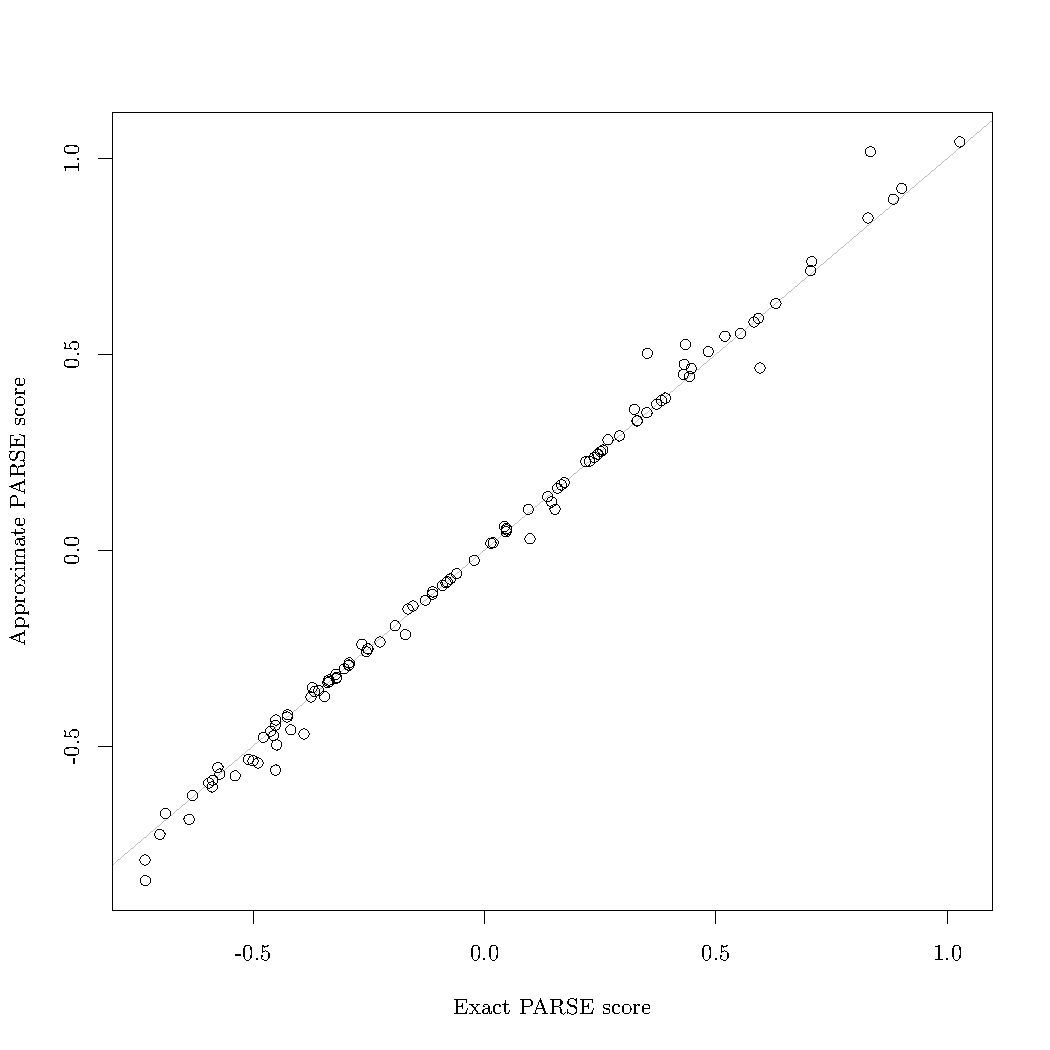
\includegraphics[width=.7\linewidth]{analysis/biosurv/reports/18_SIS_diag_dsd_final/figure/approx-calc-1}
\caption[Performance of the \acrshort{PARSE} score approximation]{The linear \acrshort{PARSE} score approximation $P \approx k A$ closely matches the exact version calculated using \gls{NNLS}, when evaluated on \gls{APGI} \gls{GEX} data.}\label{fig:app-parse-approx-matching}
\end{figure}

To use the approximation in practice, perform the following steps:
\begin{enumerate}
  \item Prepare a gene $\times$ sample matrix of linear expression estimates $A$, in which values for each row (gene) have been scaled to encompass the range $0$ to $1$.
  \item Subset $A$ to only the genes present in the $k$ table (below), and arrange rows of $A$ so that they exactly match the order of rows of $k$.  If genes present in $k$ are missing from $A$, insert all-zero rows for these genes into $A$.
  \item Calculate approximate \gls{PARSE} scores $P$ as $P = k A$.  This is equivalent to, for each column (sample) of $A$, multiplying each entry of the column of $A$ with the corresponding entry of $k$, and summing the results.
\end{enumerate}

The loading vector for the calculation of approximate \gls{PARSE} score, $k^T$, follows.
% latex table generated in R 3.1.1 by xtable 1.7-4 package
% Sat Mar 21 12:15:02 2015
\begin{longtable}{rr}
  \hline
 & Value \\ 
  \hline
A4GALT & 0.00418 \\ 
  A4GNT & -0.01632 \\ 
  ABHD16A & 0.00143 \\ 
  ABHD5 & 0.01227 \\ 
  ABLIM1 & -0.01392 \\ 
  ACE & -0.00556 \\ 
  ACKR3 & 0.00802 \\ 
  ACYP2 & -0.01298 \\ 
  ADH1A & -0.01845 \\ 
  ADM & 0.00122 \\ 
  AGRP & -0.00509 \\ 
  AKIP1 & 0.00545 \\ 
  AKR1A1 & -0.01321 \\ 
  ALDH5A1 & -0.02452 \\ 
  ALOX5AP & -0.00179 \\ 
  AMOT & -0.00825 \\ 
  ANGPTL2 & 0.01178 \\ 
  ANGPTL4 & 0.01365 \\ 
  ANKLE2 & 0.01205 \\ 
  ANKRD22 & -0.00941 \\ 
  ANKRD37 & 0.00474 \\ 
  ANLN & 0.04364 \\ 
  APCDD1 & 0.01244 \\ 
  APCS & 0.00602 \\ 
  ARFGAP3 & -0.01070 \\ 
  ARHGAP24 & -0.02524 \\ 
  ARHGEF19 & -0.00476 \\ 
  ARL4C & 0.02609 \\ 
  ARSD & -0.01466 \\ 
  ASPM & 0.01593 \\ 
  ATAD2 & 0.02602 \\ 
  ATF7IP2 & -0.00405 \\ 
  ATL3 & 0.00972 \\ 
  AURKB & 0.01869 \\ 
  AXIN2 & -0.01658 \\ 
  B3GALTL & 0.01113 \\ 
  BAMBI & -0.00680 \\ 
  BBS2 & 0.00587 \\ 
  BCKDK & -0.02452 \\ 
  BCL11B & -0.02161 \\ 
  BIRC5 & 0.02419 \\ 
  BOC & -0.03047 \\ 
  BTN3A1 & -0.00868 \\ 
  C1orf56 & -0.00865 \\ 
  C1QTNF6 & 0.01572 \\ 
  C2orf70 & -0.01360 \\ 
  C5orf46 & 0.01559 \\ 
  C9orf152 & -0.02152 \\ 
  CA8 & -0.01129 \\ 
  CACHD1 & -0.01313 \\ 
  CADPS2 & -0.02136 \\ 
  CAMK1G & -0.01790 \\ 
  CAPN6 & -0.02615 \\ 
  CARHSP1 & -0.01515 \\ 
  CATSPER1 & 0.00163 \\ 
  CAV1 & 0.02989 \\ 
  CCDC88A & 0.01480 \\ 
  CCL19 & -0.01715 \\ 
  CCNB1 & 0.03071 \\ 
  CCR7 & -0.01775 \\ 
  CD70 & 0.00954 \\ 
  CDA & 0.02792 \\ 
  CDC45 & 0.01256 \\ 
  CDK12 & -0.01624 \\ 
  CDK2 & 0.01546 \\ 
  CEBPB & 0.00404 \\ 
  CEP55 & 0.03755 \\ 
  CFDP1 & -0.00617 \\ 
  CHAF1B & 0.00920 \\ 
  CHEK1 & 0.03669 \\ 
  CHN2 & -0.02051 \\ 
  CIDEC & -0.00596 \\ 
  CIDECP & -0.00684 \\ 
  CKAP2L & 0.03545 \\ 
  CLEC3B & -0.01500 \\ 
  CNIH3 & 0.01413 \\ 
  CNNM1 & -0.01611 \\ 
  COL12A1 & 0.04098 \\ 
  COL5A3 & 0.03177 \\ 
  COL7A1 & 0.01688 \\ 
  COLGALT1 & 0.02272 \\ 
  COLGALT2 & -0.00903 \\ 
  COX4I2 & -0.00943 \\ 
  CSNK1D & -0.01128 \\ 
  CST6 & 0.02032 \\ 
  CTSL & -0.01263 \\ 
  CTSV & 0.00987 \\ 
  CYP2S1 & -0.01044 \\ 
  DCAF8 & -0.02374 \\ 
  DCBLD2 & 0.03351 \\ 
  DCUN1D5 & 0.02056 \\ 
  DENND1A & 0.01898 \\ 
  DERA & 0.01568 \\ 
  DHRS9 & -0.00454 \\ 
  DKK1 & 0.00649 \\ 
  DNAJC9 & 0.01385 \\ 
  DPY19L1 & 0.00749 \\ 
  DSG2 & 0.01463 \\ 
  DSG3 & 0.02070 \\ 
  DYNC2H1 & -0.01537 \\ 
  E2F7 & 0.03923 \\ 
  EDIL3 & 0.01326 \\ 
  EIF2AK3 & -0.02073 \\ 
  ELMOD3 & -0.03300 \\ 
  EMP3 & 0.01550 \\ 
  ENO2 & 0.02998 \\ 
  EPHX2 & -0.02392 \\ 
  ERRFI1 & 0.01597 \\ 
  EXOSC8 & -0.00850 \\ 
  EYA3 & 0.02671 \\ 
  FAH & 0.01035 \\ 
  FAM120AOS & -0.00980 \\ 
  FAM134B & -0.01945 \\ 
  FAM189A2 & -0.01692 \\ 
  FAM83A & 0.01202 \\ 
  FAM91A1 & 0.01341 \\ 
  FBXO22 & 0.00649 \\ 
  FBXW8 & -0.00891 \\ 
  FEM1B & 0.04785 \\ 
  FER & 0.02675 \\ 
  FGB & -0.00252 \\ 
  FGD6 & 0.02545 \\ 
  FGG & 0.00548 \\ 
  FHDC1 & -0.01380 \\ 
  FLRT3 & 0.01416 \\ 
  FRZB & -0.03715 \\ 
  FSCN1 & 0.02159 \\ 
  FST & 0.01504 \\ 
  FYN & -0.01133 \\ 
  GAB2 & -0.03742 \\ 
  GABPB1 & 0.01929 \\ 
  GAPDH & 0.02073 \\ 
  GATA6 & -0.01780 \\ 
  GATC & 0.02661 \\ 
  GIMAP2 & -0.03176 \\ 
  GINS2 & 0.01713 \\ 
  GNPAT & -0.01458 \\ 
  GOLM1 & -0.01171 \\ 
  GPC3 & -0.02419 \\ 
  GPR176 & 0.00563 \\ 
  HIPK2 & -0.02620 \\ 
  HJURP & 0.02296 \\ 
  HRASLS2 & 0.00196 \\ 
  HSP90B1 & -0.00641 \\ 
  HSPB6 & -0.01586 \\ 
  ICAM2 & -0.00232 \\ 
  IDH2 & 0.00528 \\ 
  IFT140 & -0.02068 \\ 
  IGFBP1 & 0.00427 \\ 
  IGLL3P & -0.01241 \\ 
  IKBIP & -0.00033 \\ 
  IL1R2 & -0.00660 \\ 
  IL20RB & 0.02671 \\ 
  IL33 & -0.00991 \\ 
  ITGA5 & 0.01407 \\ 
  ITPKB & -0.01390 \\ 
  KANK4 & 0.03261 \\ 
  KCNQ3 & 0.00040 \\ 
  KCTD10 & 0.01501 \\ 
  KCTD5 & -0.01440 \\ 
  KIAA0513 & -0.02989 \\ 
  KIAA1549L & 0.01354 \\ 
  KIF14 & 0.01477 \\ 
  KIF20A & 0.02967 \\ 
  KIF2C & 0.01417 \\ 
  KLHL5 & 0.02641 \\ 
  KNTC1 & 0.02375 \\ 
  KRT17 & 0.01644 \\ 
  KRT6A & 0.01795 \\ 
  KRT6C & 0.00798 \\ 
  KRT7 & 0.01916 \\ 
  KYNU & 0.01181 \\ 
  LAMA5 & 0.00174 \\ 
  LCNL1 & -0.01571 \\ 
  LDHA & 0.04004 \\ 
  LETM2 & 0.01687 \\ 
  LGALS9B & -0.00232 \\ 
  LINC01184 & -0.01837 \\ 
  LMO3 & -0.02246 \\ 
  LMTK2 & 0.00804 \\ 
  LOC100506562 & -0.00290 \\ 
  LOX & 0.02695 \\ 
  LYNX1 & 0.00001 \\ 
  MAP3K8 & 0.00338 \\ 
  MARCKSL1 & -0.00884 \\ 
  MARS2 & -0.01442 \\ 
  MC1R & -0.02281 \\ 
  MCEMP1 & 0.00025 \\ 
  MCM10 & 0.02451 \\ 
  MCM4 & 0.02708 \\ 
  MCOLN2 & -0.01684 \\ 
  MELK & 0.02067 \\ 
  MEOX1 & -0.01961 \\ 
  MIF & 0.01560 \\ 
  MIR99AHG & -0.03712 \\ 
  MME & 0.01102 \\ 
  MRAP2 & -0.01810 \\ 
  MRPL24 & -0.01395 \\ 
  MTRNR2L1 & -0.01563 \\ 
  NACC2 & 0.00733 \\ 
  NAMPT & 0.00071 \\ 
  NCAPD2 & 0.02756 \\ 
  NCAPG & 0.04487 \\ 
  NELFE & -0.00390 \\ 
  NEURL2 & 0.01012 \\ 
  NFIA & -0.03387 \\ 
  NFIX & -0.01186 \\ 
  NMB & -0.00205 \\ 
  NPM1 & -0.01520 \\ 
  NR0B2 & -0.01468 \\ 
  NRP2 & 0.00250 \\ 
  NUP155 & 0.02330 \\ 
  OAZ1 & -0.00134 \\ 
  ORC1 & -0.00199 \\ 
  P2RY2 & 0.01288 \\ 
  P2RY8 & -0.03043 \\ 
  P4HA1 & 0.00225 \\ 
  P4HA2 & 0.01770 \\ 
  PAX8 & 0.01350 \\ 
  PAX8-AS1 & 0.00830 \\ 
  PBXIP1 & -0.01174 \\ 
  PCDH20 & -0.00861 \\ 
  PCF11 & -0.01710 \\ 
  PCOLCE2 & -0.00752 \\ 
  PDLIM7 & 0.01678 \\ 
  PEX11B & -0.02280 \\ 
  PFKFB4 & 0.00525 \\ 
  PGAM5 & 0.00973 \\ 
  PGBD3 & 0.01700 \\ 
  PHACTR3 & 0.00172 \\ 
  PHLDA1 & 0.03330 \\ 
  PHOSPHO2 & -0.02129 \\ 
  PIGL & 0.00833 \\ 
  PLAC9 & -0.02093 \\ 
  PLAU & 0.03213 \\ 
  PLEKHS1 & -0.01672 \\ 
  PLIN2 & -0.01174 \\ 
  PLIN3 & -0.00506 \\ 
  PLOD1 & 0.00369 \\ 
  PLOD2 & 0.02261 \\ 
  POC1A & 0.01507 \\ 
  POLA2 & 0.00692 \\ 
  POP5 & -0.00224 \\ 
  POU2AF1 & -0.02222 \\ 
  PP7080 & -0.01242 \\ 
  PPAPDC1A & 0.02867 \\ 
  PPM1H & -0.02311 \\ 
  PPP1R12B & 0.00096 \\ 
  PPP1R14B & 0.01352 \\ 
  PPP1R3C & 0.00125 \\ 
  PPY & -0.02787 \\ 
  PRC1 & 0.02492 \\ 
  PRDM16 & -0.02289 \\ 
  PREP & -0.01799 \\ 
  PRKCDBP & 0.00755 \\ 
  PRMT7 & -0.01665 \\ 
  PROSER2 & 0.01761 \\ 
  PRR11 & 0.01859 \\ 
  PTGES & 0.02681 \\ 
  PTPN21 & 0.01723 \\ 
  PXDN & 0.02281 \\ 
  PYGL & 0.01714 \\ 
  RAB31 & 0.01316 \\ 
  RACGAP1 & 0.02957 \\ 
  RALGAPB & 0.02214 \\ 
  RAP1GAP & -0.03483 \\ 
  RASL11B & -0.01808 \\ 
  RAVER2 & -0.01352 \\ 
  RBMS2 & 0.02834 \\ 
  RERE & -0.01635 \\ 
  RERGL & -0.01801 \\ 
  RFC5 & 0.01848 \\ 
  RFK & -0.01090 \\ 
  RFX2 & -0.00264 \\ 
  RGS3 & -0.00319 \\ 
  RGS5 & -0.01505 \\ 
  RHOF & 0.02828 \\ 
  RMND5A & -0.00614 \\ 
  RNF103 & -0.03019 \\ 
  RPA2 & -0.02756 \\ 
  RPIA & -0.02226 \\ 
  SAMD5 & -0.00655 \\ 
  SCGB2A1 & -0.01773 \\ 
  SCYL2 & 0.01826 \\ 
  SDIM1 & -0.01083 \\ 
  SEC23IP & -0.01125 \\ 
  SELENBP1 & -0.02707 \\ 
  SEPW1 & -0.01161 \\ 
  SERPINB3 & -0.00201 \\ 
  SERPINH1 & 0.02086 \\ 
  SERTAD2 & -0.00995 \\ 
  SGSM1 & -0.02933 \\ 
  SH3GL1 & -0.02784 \\ 
  SLAMF9 & -0.00761 \\ 
  SLC12A2 & -0.01821 \\ 
  SLC15A1 & -0.00139 \\ 
  SLC16A3 & 0.01842 \\ 
  SLC2A1 & 0.01424 \\ 
  SLC2A3 & 0.00438 \\ 
  SLC30A3 & -0.01126 \\ 
  SLC40A1 & -0.02146 \\ 
  SMOX & -0.02258 \\ 
  SNORA11D & -0.00256 \\ 
  SNRPB & 0.00276 \\ 
  SOBP & -0.03269 \\ 
  SOD2 & 0.00120 \\ 
  SPHK1 & 0.03861 \\ 
  SPIN4 & 0.01254 \\ 
  SPOCD1 & 0.02117 \\ 
  SPOCK1 & 0.03046 \\ 
  SPP1 & 0.00175 \\ 
  ST3GAL2 & -0.02187 \\ 
  ST6GAL1 & -0.02118 \\ 
  ST6GALNAC1 & -0.01232 \\ 
  STAT5B & -0.03172 \\ 
  STK39 & -0.01196 \\ 
  SUGCT & 0.01833 \\ 
  SULF2 & 0.01494 \\ 
  SYNE2 & -0.00968 \\ 
  TAF5L & -0.01213 \\ 
  TARBP2 & -0.01019 \\ 
  TCEA3 & -0.02679 \\ 
  TCTA & -0.03326 \\ 
  TGFBI & 0.03259 \\ 
  THSD7B & -0.01931 \\ 
  TLE4 & -0.01794 \\ 
  TM9SF3 & -0.01255 \\ 
  TMED1 & -0.01796 \\ 
  TMEM26 & 0.03659 \\ 
  TMTC4 & -0.01797 \\ 
  TNFRSF10D & -0.00315 \\ 
  TNFRSF17 & -0.01180 \\ 
  TNFRSF6B & 0.02308 \\ 
  TOM1 & -0.01640 \\ 
  TOM1L2 & 0.00266 \\ 
  TOR2A & -0.02926 \\ 
  TPD52L2 & -0.00579 \\ 
  TPX2 & 0.02590 \\ 
  TRAPPC2 & -0.01920 \\ 
  TREM1 & -0.00073 \\ 
  TRERF1 & 0.00581 \\ 
  TRIM2 & -0.02689 \\ 
  TSTD1 & -0.02503 \\ 
  TUBA1C & 0.02053 \\ 
  TWIST1 & 0.02246 \\ 
  UFC1 & -0.03123 \\ 
  UHRF2 & 0.01445 \\ 
  UPP1 & 0.00182 \\ 
  USP30 & 0.00629 \\ 
  VPS35 & -0.01219 \\ 
  VSTM2L & 0.00352 \\ 
  WNT2B & -0.00812 \\ 
  XXYLT1 & 0.00341 \\ 
  ZBED2 & 0.02396 \\ 
  ZFPM1 & -0.02180 \\ 
  ZNF185 & 0.01435 \\ 
  ZNF565 & -0.00565 \\ 
  ZNF658 & -0.01988 \\ 
  ZPLD1 & 0.00165 \\ 
  ZSCAN16 & -0.00720 \\ 
  ZSCAN32 & -0.02184 \\ 
   \hline
\hline
\end{longtable}

